\documentclass[conference]{IEEEtran}
\IEEEoverridecommandlockouts
% 1. Load essential math packages FIRST
\usepackage{amsmath,amssymb,amsfonts}
\usepackage{algorithmic}
% 2. Load other English-support packages
\usepackage{cite}
\usepackage{graphicx}
\usepackage{textcomp}
\usepackage{xcolor}
\usepackage{array}
\usepackage{booktabs}
\usepackage{tabularx}
\usepackage{algorithm}
\usepackage{pdflscape}   % For landscape orientation
\usepackage{multirow}    % For multi-row cells (if needed)
\usepackage{stfloats} % Add to preamble
\usepackage{fancyhdr}
\usepackage{lastpage}
\usepackage{tikz}
% 3. Configure fonts with proper Arabic features
\usepackage{fontspec}
\setmainfont{Times New Roman}
\newfontfamily\arabicfont[
  Script=Arabic,
  Scale=1.0,
  Renderer=HarfBuzz,
  RawFeature={+ss05,+ss06,+ss07}
]{Amiri}

% 4. Define \arb command with proper RTL directionality
\newcommand{\arb}[1]{%
  \bgroup
  \arabicfont
  \textdir TRT
  \pardir TRT
  #1%
  \egroup
}

% \newfontfamily\hafsFont{UthmanicHafs}[
%     Script=Arabic,
%     Path=./fonts/UthmanicHafs/,
%     Scale=1.1,
%     Extension = .ttf,
%     UprightFont=*-Regular,
%     % BoldFont=*-Bold,
%     % ItalicFont=*-Italic,
%     % BoldItalicFont=*-BoldItalic
% ]
%
% \newcommand{\hafs}[1]{{\hafsFont\arb{#1}}}
% 5. Load hyperref LAST
\usepackage{hyperref}
\hypersetup{
    colorlinks=true,
    linkcolor=blue,
    filecolor=magenta,      
    urlcolor=cyan,
    pdfencoding=unicode,
}
% Fix section numbering
\makeatletter
\def\@seccntformat#1{\csname the#1\endcsname\quad}
\makeatother
\def\BibTeX{{\rm B\kern-.05em{\sc i\kern-.025em b}\kern-.08em
    T\kern-.1667em\lower.7ex\hbox{E}\kern-.125emX}}
% Footer configuration
\pagestyle{fancy}
\fancyhf{}
\renewcommand{\headrulewidth}{0pt}
\renewcommand{\footrulewidth}{0pt}
    
\begin{document}
\title{Automatic Pronunciation Error Detection and Correction of the Holy Quran's Learners Using Deep Learning\\
}
\author{\IEEEauthorblockN{Abdullah Abdelfttah}
\IEEEauthorblockA{\textit{{\footnotesize Computer and Systems Engineering }} \\
\textit{{\footnotesize Faculty of Engineering Ain Shams University}}\\
{\footnotesize Cairo, Egypt} \\
2101398@eng.asu.edu.eg}
\and
\IEEEauthorblockN{Mahmoud I. Khalil}
\IEEEauthorblockA{\textit{{\footnotesize Computer and Systems Engineering }} \\
\textit{{\footnotesize Faculty of Engineering Ain Shams University}}\\
{\footnotesize Cairo, Egypt} \\
mahmoud.khalil@eng.asu.edu.eg}
\and
\IEEEauthorblockN{Hazem Abbas}
\IEEEauthorblockA{\textit{{\footnotesize Computer and Systems Engineering }} \\
\textit{{\footnotesize Faculty of Engineering Ain Shams University}}\\
{\footnotesize Cairo, Egypt} \\
hazem.abbas@eng.asu.edu.eg}
}
\maketitle
\begin{abstract}
	Assessing spoken language is challenging, and quantifying pronunciation metrics for machine learning models is even harder. However, for the Holy Quran, this task is enabled by the rigorous recitation rules (tajweed) established through the efforts of Muslim scholars, making highly effective assessment possible. Despite this advantage, scarcity of high-quality annotated data remains a significant barrier. In this work, we bridge these gaps by introducing: (1) A 98\% automated pipeline to produce high-quality Quranic datasets – encompassing: Collection of recitations from expert reciters, Segmentation at pause points (waqf) using our fine-tuned wav2vec2-BERT model, Transcription of segments, Transcript verification via our novel Tasmeea algorithm; (2) 850+ hours of audio (~300K annotated utterances); (3) \textbf{qdat\_bench} benchmarks phonemes, diacritization, and Tajweed rules (Ghunnah, Qalqalah, Madd) on real recitation errors containing 159 samples; (4) A novel ASR-based approach for pronunciation error detection, utilizing our custom Quran Phonetic Script (QPS) to encode Tajweed rules (unlike the IPA standard for Modern Standard Arabic). QPS uses an 11-level script: (Phoneme level): Encodes Arabic letters with short/long vowels. (Sifat level): Encodes articulation characteristics of every phoneme. We further include comprehensive modeling with our novel multi-level CTC Model which achieved 0.21\% and 1.94\% average Phoneme Error Rate (PER) on the testset and qdat\_bench respectively, with 75.8\% Tajweed F1 score and 84.7\% accuracy on the benchmark. We release all code, data, and models as open-source: \href{https://obadx.github.io/quran-muaalem/en/}{https://obadx.github.io/quran-muaalem/en/}


\end{abstract}
\begin{IEEEkeywords}
	Mispronunciation Detection Model, Arabic Natural Language Processing, End-to-end Models
\end{IEEEkeywords}
\section{Introduction}
Assessing pronunciation is not a simple task \cite{kheir2023automatic}, as it does not only rely on pronouncing phonemes correctly but also involves other factors like intonation, prosody, and stress. Does learning these mean one is done? No---other factors include fluency and completeness \cite{kheir2023automatic}. However, the Holy Quran presents unique characteristics: it is among the easiest spoken texts to learn despite containing special phonemes absent in other languages.

The pronunciation of the Holy Quran is governed by rigorously strict rules formally defined by ancient Muslim scholars since the 6th century. Despite their beauty and precision, these rules have not been comprehensively digitized (to our knowledge) for Quranic pronunciation assessment.

Although RDI pioneered computer-aided Quranic instruction \cite{sherif2007enhancing}, they neither disclosed their phoneticization process nor released data/models. Consequently, new research must start from basics: defining phoneticization, data, and models. To bridge this gap, we introduce:

\begin{itemize}
	\item \textbf{A Phonetizer}: Encodes \emph{all} Tajweed rules and articulation attributes (\emph{Sifat}) defined by classical scholars, except \emph{Ishmam} (\arb{إشمام})
	\item \textbf{A 98\% automated pipeline}: Generates highly accurate datasets from expert recitations
	\item \textbf{A dataset}: $\sim$300K annotated utterances (850+ hours)
	\item \textbf{qdat\_bench}: Benchmarks phonemes, diacritization, and Tajweed rules (Ghunnah, Qalqalah, Madd) on real recitation errors containing 159 samples
	\item \textbf{Integration}: Our multi-level CTC model proves the Quranic phonetic script is learnable (0.21\% average phoneme error rate)
\end{itemize}

The paper is organized as follows:
\begin{itemize}
	\item \textbf{Related Work}: Expands on strengths/weaknesses of prior research
	\item \textbf{Quran Phonetic Script}: Introduces our two-level script: \textbf{phonemes} and \textbf{Sifat} (10 attributes $\to$ 11 total levels)
	\item \textbf{Data Pipeline}: Stages include:
	      \begin{enumerate}
		      \item Digitized Quran script as foundation
		      \item \emph{Hafs} methodology criteria
		      \item Expert recitation collection
		      \item Segmentation at pause points (\arb{وقف})
		      \item Segment transcription
		      \item Validation via \emph{Tasmee} (\arb{تسميع}) algorithm
	      \end{enumerate}
	\item \textbf{Modeling}: Demonstrates learnability of the phonetic script
	\item \textbf{Results}: Analysis of outcomes
	\item \textbf{Limitations \& Future Work}: Next research directions
	\item \textbf{Conclusion}: Summary of contributions
	\item \textbf{Appendix}: Details on \emph{Mushaf} attributes and algorithms
\end{itemize}


\section{Related Work}

\subsection{Quran Pronunciation Datasets}
We discuss the most important datasets here. everyayah\footnote{\url{everyayah.com}} is the largest openly available dataset with 26 complete \emph{Mushafs} segmented and annotated by Ayah by experts like Al Hossary and non-experts such as Fares Abbad. Qdat \cite{osman2021qdat} contains 1509 utterances of single specific Ayahs labeled for three rules: Madd, Ghunna, and Ikhfaa. Although the scale is relatively small, it was widely adopted by the community \cite{10092350}, and \cite{shaiakhmetov2025evaluation} due to being open-source. The Tarteel v1 dataset \cite{khan2021tarteel} consists of 25K utterances with diacritics and no Tajweed rules. The latter is the Tarteel\footnote{\url{tarteel.ai}} private dataset, a massive 9K-hour collection annotated with diacritics without Tajweed rules. The most recent benchmark is IqraaEval \cite{kheir2025towards}, which presents a test set of 2.2 hours from 18 speakers, but uses Modern Standard Arabic (MSA) without Tajweed rules.

\subsection{Quran Pronunciation Models}
To our knowledge, the first work addressing automated pronunciation assessment for the Holy Quran is RDI \cite{sherif2007enhancing}, which built a complete system for detecting pronunciation errors. The work does not specify which errors were included or excluded but mentions testing Qalqala, Idgham, and Iqlab rules. It also omits details on Quranic word phoneticization. Subsequent work continued with \cite{abdou2014computer} and \cite{al2018computer}, using Deep Neural Networks (DNNs) to replace HMMs and improve the system. Many studies rely on modeling phoneme duration for duration-dependent rules like Madd and Ghunna, e.g., \cite{mohammed2017recognition}, \cite{alqadasi2023improving}, but use limited datasets and focus on specific verses rather than the entire Quran. Others concentrate on detecting specific rules like Qalqala \cite{10092350} or Ghunna and Madd \cite{shaiakhmetov2025evaluation}, \cite{10485145}. However, most efforts except RDI work train on small-scale datasets from specific Quranic chapters.

At this point, Tarteel emerges; though lacking Tajweed rules, they built a robust ASR system for diacritized character detection. They developed a crowd-sourced dataset \cite{khan2021tarteel} of 25K utterances (68 hours), later extended via application users to 9K hours of private annotated data. The work most aligned with our vision of detecting all error types (including Tajweed and \emph{Sifat}/articulation attributes) is \cite{putra2012developing}. Although it relies on HMMs and minimal data, it introduces a multi-level detection system: \emph{Makhraj} (phoneme level) and Tajweed rules level.

\subsection{Pretrained Speech Encoders with Self-Supervised Learning (SSL)}
Speech pretraining began early \cite{hinton2006reducing} but was constrained by the sequential nature of Recurrent Neural Networks (RNNs) \cite{hopfield1982neural}. The rise of Transformers \cite{vaswani2017attention} facilitated greater GPU parallelization, enabling large-scale pretraining. BERT \cite{devlin2019bert} using Masked Language Modeling (MLM) introuduce large unsuprvised pretraing which has better results on down stream taks. This soon extended to speech with wav2vec \cite{schneider2019wav2vec} and wav2vec2.0, which added product quantization \cite{baevski2020wav2vec}. Conformer later replaced vanilla Transformers for speech by integrating convolution \cite{gulati2020conformer}. Google's Wav2Vec2-BERT \cite{chung2021w2v} then applied MLM to speech. Finally, Facebook extended Wav2Vec2-BERT pretraining \cite{barrault2023seamless} to 4.5M hours (including 110K Arabic hours), ideal for low-resource language fine-tuning.



\section{Quran Phonetic Script}
\label{sec:qps}
We consider the Quran Phonetic Script to be the most valuable and important contribution of our work. By formalizing the assessment of Holy Quran pronunciation as an ASR problem represented through this script, we provide a comprehensive solution to the task.

\subsection{Motivation for Developing Quran Phonetic Script}
Modern Standard Arabic (MSA) orthography cannot adequately represent Tajweed rules for error detection. For example, MSA cannot measure the precise length of Madd rules. Previous research (e.g., \cite{omran2023automatic}) focused on single rules like Qalqalah. Our phonetic script addresses this limitation by capturing all Tajweed pronunciation errors except Ishmam (\arb{إشمام}), which involves a visual mouth movement without audible output.

\subsection{Background}
We based our script on classical Muslim scholarship rather than the International Phonetic Alphabet (IPA) for these reasons:

\begin{enumerate}
    \item \textbf{Historical Precedence}: Muslim scholars from the 6th to 14th centuries rigorously defined Quranic errors centuries before modern phonetics emerged in the West.
    \item \textbf{Scientific Foundation}: Scholars like Al-Khalil ibn Ahmad (6th century AH) systematically described articulations and attributes with remarkable accuracy comparable to modern phonetics \cite{article-khalil}.
    \item \textbf{Pedagogical Relevance}: Learners' errors align with classical definitions according to expert Quran teachers.
\end{enumerate}

\subsection{Defining Mistakes in Quran Recitation}
Following \cite{sweed2021}, Quran recitation errors fall into three categories:
\begin{itemize}
    \item \textbf{Articulation Errors}: Incorrect pronunciation of phonemes
    \item \textbf{Attribute Errors}: Mistakes in letter characteristics (Sifat al-Huruf)
    \item \textbf{Tajweed Rule Errors}: Incorrect application of rules like Ghunnah, Madd, etc.
\end{itemize}

Our script comprehensively addresses all three aspects through two output levels:
\begin{itemize}
    \item \textbf{Phonemes Level}: Represents letters, vowels, and Tajweed rules
    \item \textbf{Sifat Level}: Represents articulation attributes for each phoneme
\end{itemize}

Refer to tables: \ref{tab:phoneme_set} \ref{tab:sifat_set} for Phonemes and Sifat levels.

\subsection*{Key Design Principles}
\begin{enumerate}
    \item \textbf{Madd Representation}:
    \begin{itemize}
        \item Normal Madd appears as consecutive madd symbols (e.g., 4-beat Madd: \arb{اااا})
        \item Madd al-Leen represented with multiple waw/yaa symbols
    \end{itemize}
    
    \item \textbf{Emphatic Articulation}:
    \begin{itemize}
        \item Stressed Ghunnah (e.g., \arb{النون المشددة}) as three consecutive noon symbols (\arb{ننن})
        \item Ikhfa represented as three consecutive noon\_mokhfah (\arb{ںںں}) or meem\_mokhfah (\arb{۾۾۾})
    \end{itemize}
    
    \item \textbf{Idgham Handling}:
    \begin{itemize}
        \item Assimilation represented by doubling (e.g., \arb{مَن يَعْمَلْ} $\rightarrow$ \arb{مَيييَعمَل})
    \end{itemize}
    
    \item \textbf{Special Cases}:
    \begin{itemize}
        \item Sakin: No following symbol
        \item Imala: fatha\_momala and alif\_momala
        \item Rawm: dama\_mokhtalasa marker
    \end{itemize}
\end{enumerate}

Example: In table~\ref{tab:examples_with_sifat} shows how our phonetizer works.





\begin{table*}[h]
\centering
\caption{Examples of Uthmani to Phonetic Script Conversion with Sifat Attributes}
\label{tab:examples_with_sifat}
\scriptsize
\setlength{\tabcolsep}{3pt}
\begin{tabular}{@{}>{\centering\arraybackslash}m{1.2cm} >{\centering\arraybackslash}m{1.5cm} *{10}{>{\centering\arraybackslash}m{0.7cm}@{}}}
\toprule
\textbf{Uthmani} & \textbf{Phonetic} & 
\textbf{H/J} & 
\textbf{S/R} & 
\textbf{T/T} & 
\textbf{Itb} & 
\textbf{Saf} & 
\textbf{Qal} & 
\textbf{Tik} & 
\textbf{Taf} & 
\textbf{Ist} & 
\textbf{Gho} \\
\cmidrule(lr){1-1} \cmidrule(lr){2-2} \cmidrule(lr){3-12}
\arb{أَ} & \arb{ءَ} & jahr & shd & mrq & mnf & no & nql & nkr & ntf & nst & nmg \\
\arb{تُ} & \arb{تُ} & hams & shd & mrq & mnf & no & nql & nkr & ntf & nst & nmg \\
\arb{حَـ} & \arb{حَ} & hams & rkh & mrq & mnf & no & nql & nkr & ntf & nst & nmg \\
\arb{ـٰٓ} & \arb{اااااا} & hams & rkh & mrq & mnf & no & nql & nkr & ntf & nst & nmg \\
\arb{جُّ} & \arb{ججُ} & jahr & shd & mrq & mnf & no & nql & nkr & ntf & nst & nmg \\
\arb{وٓ} & \arb{ۥۥۥۥۥۥ} & jahr & rkh & mrq & mnf & no & nql & nkr & ntf & nst & nmg \\
\arb{نِّ} & \arb{ننننِ} & jahr & btw & mrq & mnf & no & nql & nkr & ntf & nst & mg \\
\arb{ى} & \arb{ۦۦ} & jahr & rkh & mrq & mnf & no & nql & nkr & ntf & nst & nmg \\
\bottomrule
\end{tabular}

\vspace{2mm}
\begin{center}  % Centering wrapper added here
\scriptsize
Phonetization of word (\hafs{أَتُحَٰٓجُّوٓنِّى}) \\
\textbf{Attribute Abbreviations:} \\
H/J: Hams/Jahr \quad S/R: Shidda/Rakhawa \quad T/T: Tafkheem/Taqeeq \quad Itb: Itbaq \\
Saf: Safeer \quad Qal: Qalqla \quad Tik: Tikraar \quad Taf: Tafashie \quad Ist: Istitala \quad Gho: Ghonna \\

\textbf{Value Abbreviations:} \\
shd: shadeed \quad rkh: rikhw \quad btw: between \quad mrq: moraqaq \\
mof: mofakham \quad mnf: monfateh \quad mtb: motbaq \quad no: no\_safeer \\
nql: not\_moqalqal \quad nkr: not\_mokarar \quad ntf: not\_motafashie \\
nst: not\_mostateel \quad nmg: not\_maghnoon \quad mg: maghnoon
\end{center}  % End of centering wrapper
\end{table*}


\subsection{Development Methodology}
Our phonetization has two steps:
\begin{enumerate}
    \item \textbf{Imlaey to Uthmani Conversion} \\
    We selected Uthmani script as our foundation because:  
    \begin{itemize}
        \item Contains specialized Tajweed diacritics (Madd, Tasheel, etc.)
        \item Preserves pause rules critical for recitation (e.g., stopping on \arb{رحمت})
    \end{itemize}
    
    In order to do that, we created an annotation UI to manually annotate misaligned words in both scripts. For example \ref{tab:imlaey_to_uthmani_ex}, after that, we developed an algorithm that relies on the annotations to convert Imlaey to Uthmani.
    \item \textbf{Uthmani to Phonetic Script Conversion} \\
We implemented the process through 26 sequential operations. Each operation contains one or more regular expressions, as shown in the Appendix~\ref{subsec:conversion_ops}.

    \item \textbf{Extracting Sifat}: Next, we extract the 10 attributes (Sifat) defined in Table~\ref{tab:sifat_set}, excluding \textbf{Inhiraf} (\arb{إنحراف}), as it describes the shidda/rakhawa spectrum, and \textbf{Leen} (\arb{اللين}), as it was already handled through our Madd representation.
\end{enumerate}

\begin{table}[h]
\caption{Example of misalignment between Uthmani and Imlaey Scripts}
\label{tab:imlaey_to_uthmani_ex}
\centering
\begin{tabular}{|c|c|}
    \hline
    \textbf{Imlaey Script} & \textbf{Uthmani Script} \\
    \hline
    \arb{يَا ابْنَ أُمَّ} & \arb{يَبْنَؤُمَّ} \\
    \hline
\end{tabular}
\end{table}



\section{Data Preparation}
To prepare the data, we first defined selection criteria. We aimed to collect recitations from the best reciters worldwide to serve as references for judging Quran learners. In our study, we considered only \textit{Hafs} riwayah (\arb{رواية حفص}) as it's the most popular recitation method globally. Recognizing that manual data annotation requires significant effort and time, we created a 98\% automated pipeline for data collection. The steps are:
(1) Choose a digitized Quran script as the project foundation.
(2) Define criteria for \textit{Hafs} methodology.
(3) Collect expert recitations
(4) Segment recitations at pause points (\arb{وقف})
(5) Transcribe segments.
(6) Validate data through \textit{Tasmee} (\arb{تسميع}) Algorithm.
(7) Develop Quran Phonetic Script.

We define a \textit{Moshaf} as a complete Quran recitation (chapters 1-114) by a specific reciter. Statistics are summarized in table~\ref{tab:moshaf}. We manually annotated 5400 samples out of 286,537 utterances, resulting for the automation ratio of 98\%.

\begin{table}[htbp]
	\centering
	\caption{Dataset Statistics per Moshaf}
	\label{tab:moshaf}
	\begin{tabular}{ccc}
		\hline
		\textbf{Moshaf ID} & \textbf{Hours}       & \textbf{Length} \\
		\hline
		0.0                & 28.48          & 9133            \\
		0.1                & 40.31          & 10764           \\
		0.2                & 49.47          & 9971            \\
		0.3                & 37.19          & 12604           \\
		1.0                & 28.41          & 10939           \\
		2.0                & 51.05          & 9942            \\
		2.1                & 30.03          & 10394           \\
		3.0                & 25.19          & 10444           \\
		4.0                & 29.12          & 10994           \\
		5.0                & 28.02          & 11482           \\
		6.0                & 39.39          & 12435           \\
		7.0                & 28.26          & 9907            \\
		8.0                & 30.86          & 10330           \\
		9.0                & 27.95          & 10642           \\
		11.0               & 24.01          & 10363           \\
		12.0               & 33.42          & 9880            \\
		13.0               & 33.99          & 9377            \\
		19.0               & 30.11          & 11278           \\
		22.0               & 28.11          & 10332           \\
		24.0               & 28.51          & 9868            \\
		25.0               & 16.93          & 7922            \\
		26.0               & 30.44          & 11565           \\
		26.1               & 32.71          & 11850           \\
		27.0               & 28.05          & 11213           \\
		28.0               & 31.05          & 10535           \\
		29.0               & 27.79          & 11061           \\
		30.0               & 29.14          & 11312           \\
		\hline
		\textbf{Total}     & \textbf{847.9944402} & \textbf{286537} \\
		\hline
	\end{tabular}
\end{table}

\subsection{Choose a Digitized Version of the Holy Quran}
The Quran has multiple digitized versions including Tanzil\footnote{\url{https://tanzil.net}} and King Fahd Complex\footnote{\url{https://qurancomplex.gov.sa}}. We chose Tanzil because:
\begin{itemize}
	\item It uses standard Unicode characters
	\item Contains both \textit{Imlaei} and \textit{Uthmani} versions
	\item Maintains high accuracy
\end{itemize}
We excluded KFGQPC due to its evolving/unstable nature compared to Tanzil.

\subsection{Define Variant Criteria for Hafs}
\textit{Hafs} riwayah contains variants, e.g., \textit{Madd Al-Munfasil} (\arb{مد المنفصل}) can extend 2, 4, 5, or 6 beats. We rigorously defined these variants through the Qira'at literature \cite{al-dabbaa}, summarized in the following attributes in the Appendix section \ref{sec:moshaf_attributes}.


\subsection{Collect Expert Recitations}
We collected recitations from 22 world-class reciters with premium audio quality, totaling \textbf{893 hours} pre-filtering.

\begin{figure}[htbp]
	\centering
	\includegraphics[width=0.8\linewidth]{figures/stats.png}
	\caption{Database Collection Statistics}
	\label{fig:stats}
\end{figure}

\begin{figure}[htbp]
	\centering
	\includegraphics[width=0.8\linewidth]{figures/reciter.png}
	\caption{Reciters Statistics}
	\label{fig:reciters}
\end{figure}

We developed a web GUI using Streamlit\footnote{\url{https://streamlit.io/}} that:
\begin{itemize}
	\item Downloads and extracts metadata for each track
	\item Organizes data by Moshaf (each chapter as "001.mp3")
	\item Annotates Moshaf attributes
\end{itemize}

\subsection{Segment Recitations}
Since Tajweed rules are affected by pauses (\arb{وقف}), accurate segmentation is crucial. We initially tested open-source Voice Activity Detection (VAD) models including SileroVAD \cite{SileroVAD} and PyAnnotate \cite{Plaquet23}. Poor Quran-specific performance led us to develop a custom segmenter by fine-tuning Wav2Vec2-BERT \cite{barrault2023seamless} for frame-level classification.

\subsubsection{Preparing Segmenter Data}
We selected mosahf compatible with SileroVAD v4, using EveryAyah\footnote{\url{https://everyayah.com/}} (pre-segmented by ayah) as ground truth. After tuning parameters per Moshaf:
\begin{itemize}
	\item Threshold
	\item Minimum silence duration (merges segments)
	\item Minimum speech duration (discards short segments)
	\item Padding (added at segment boundaries)
\end{itemize}

\paragraph{Data Augmentation}
Using the Audiomentations \cite{Audiomentations} library, we replicated SileroVAD's noise setup on 40\% of samples, adding:
\begin{itemize}
	\item \texttt{TimeStretch} (0.8x-1.5x) to simulate recitation speeds
	\item Sliding window truncation (1-second windows) for long samples instead of exclusion
\end{itemize}

\subsubsection{Training Segmenter}
We fine-tuned Wav2Vec2-BERT for frame classification (1 epoch):

% \begin{figure}[htbp]
% \centering
% \includegraphics[width=\linewidth]{figures/vad-arch.png}
% \caption{VAD architecture vs. standard streaming models}
% \label{fig:vad-arch}
% \end{figure}

\begin{figure*}[b]
	\centering
	\includegraphics[width=0.85\textwidth]{figures/vad-arch.png}
	\caption{VAD architecture vs. standard streaming models}
	\label{fig:vad-arch}
\end{figure*}

Results of our segmenter on unseen mosahf in table~\ref{tab:seg_results}:

\begin{table}[htbp]
	\label{tab:seg_results}
	\centering
	\caption{Test results of the segmenter on unseen full moshaf. The result is validated by actual usage of the segmenter}
	\vspace{2pt}
	\begin{tabular}{lc}
		\hline
		\textbf{Metric} & \textbf{Value} \\
		\hline
		Test Loss       & 0.0277         \\
		Test Accuracy   & 0.9935         \\
		Test F1 Score   & 0.99476        \\
		\hline
	\end{tabular}
\end{table}

\subsection{Transcribe Segmented Parts}
We employed Tarteel ASR \cite{tarteel_whisper_ar_quran} (Whisper fine-tuned on Quranic recitations \cite{radford2023robust}). To handle its 30-second limit, we used sliding window truncation (10-second windows), with verification in the next step.

\subsection{Verification of Segmentation and Transcription}
\textbf{Segmentation Verification}: Manual inspection of 50-75 random samples per Moshaf. Moshaf 25.0 was excluded due to poor segmentation.

\textbf{Transcription Verification}: \textit{Tasmeea}-inspired algorithm:
(1) Match segments to Quranic text.
(2) Identify missing surah parts.
(3) Manual correction.

Refer to the Tasmeea Algorithm in the Appendix \ref{alg:tasmeea}

After matching, we catalogued missing Quranic portions per surah. Then correct transcription errors identified through the above process.

\begin{figure}[htbp]
	\centering
	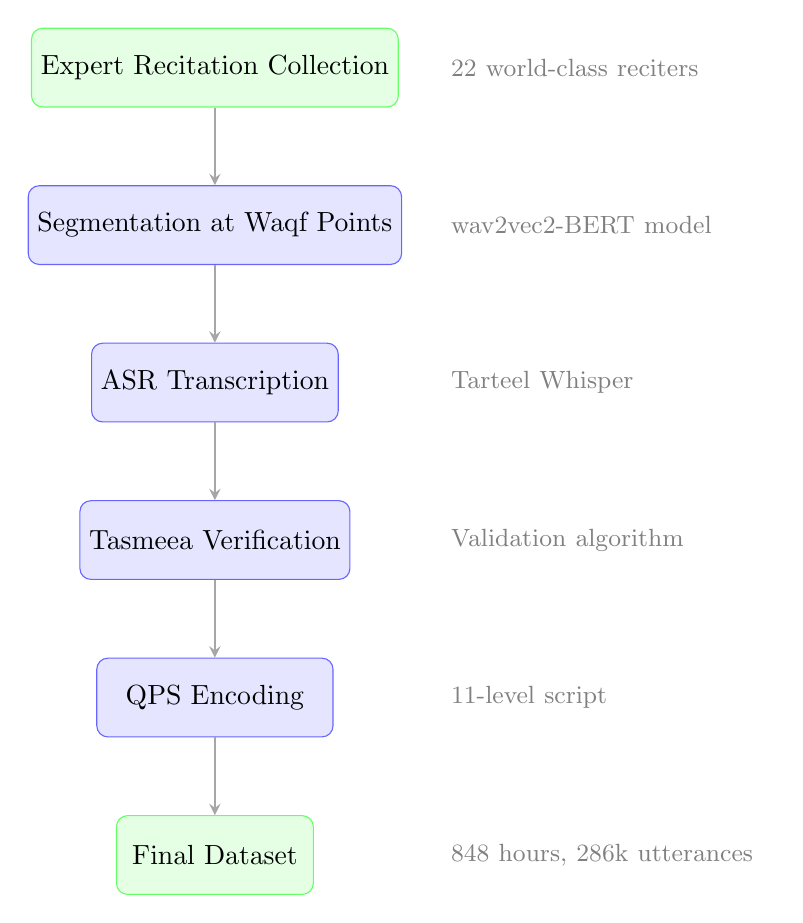
\begin{tikzpicture}[node distance=2cm, auto]
		% Define styles with simple colors
		\tikzstyle{process} = [rectangle, minimum width=3cm, minimum height=1cm, text centered, draw=blue!60, fill=blue!10, rounded corners]
		\tikzstyle{data} = [rectangle, minimum width=2.5cm, minimum height=1cm, text centered, draw=green!60, fill=green!10, rounded corners]
		\tikzstyle{arrow} = [thick,->,>=stealth,draw=gray!70]

		% Nodes
		\node[data] (collection) {Expert Recitation Collection};
		\node[process, below of=collection] (segmentation) {Segmentation at Waqf Points};
		\node[process, below of=segmentation] (transcription) {ASR Transcription};
		\node[process, below of=transcription] (verification) {Tasmeea Verification};
		\node[process, below of=verification] (encoding) {QPS Encoding};
		\node[data, below of=encoding] (dataset) {Final Dataset};

		% Arrows
		\draw[arrow] (collection) -- (segmentation);
		\draw[arrow] (segmentation) -- (transcription);
		\draw[arrow] (transcription) -- (verification);
		\draw[arrow] (verification) -- (encoding);
		\draw[arrow] (encoding) -- (dataset);

		% Side annotations
		\node[right of=collection, xshift=3cm, text width=4cm, text=gray] {\small 22 world-class reciters};
		\node[right of=segmentation, xshift=3cm, text width=4cm, text=gray] {\small wav2vec2-BERT model};
		\node[right of=transcription, xshift=3cm, text width=4cm, text=gray] {\small Tarteel Whisper};
		\node[right of=verification, xshift=3cm, text width=4cm, text=gray] {\small Validation algorithm};
		\node[right of=encoding, xshift=3cm, text width=4cm, text=gray] {\small 11-level script};
		\node[right of=dataset, xshift=3cm, text width=4cm, text=gray] {\small 848 hours, 286k utterances};
	\end{tikzpicture}
	\caption{The complete data preparation pipeline showing the six main stages from expert recitation collection to the final dataset generation. Each stage utilizes specialized models and algorithms to ensure high-quality annotations.}
	\label{fig:data_pipeline}
\end{figure}



\section{Modeling The Quran Phonetic Script}
Our Quran Phonetic script has two outputs: \texttt{phonemes} and \texttt{sifat} (which has 10 attributes). We modeled this as follows: Imagine you are given an input speech utterance and want to output transcripts in Arabic, English, French, and German simultaneously. We implemented this as a speech encoder with a linear layer for each language. Replacing languages with our 11 levels (\texttt{phonemes} and the 10 sifat), we obtain 11 parallel transcription levels. We chose CTC loss \cite{graves2006ctc} without language model integration because we aim to capture what the user actually said, not what they intended to say. We name our architecture \textbf{Multi-level CTC}.  

We compute the loss by averaging all CTC losses for the 11 levels, assigning a weight of 0.4 to the \texttt{phonemes} level as it has the largest vocabulary size (43) compared to other levels.  

\begin{figure}[htbp]
\centering
\includegraphics[width=\linewidth]{figures/multi-level-ctc.png}
\caption{Multi-level CTC loss Architecture composed of 11 Heads for every level and CTC loss for every level with weighted average loss}
\label{fig:multilevel-ctc}
\end{figure}

We fine-tuned Facebook's Wav2Vec2-Bert \cite{barrault2023seamless} for a single epoch with a constant learning rate of \texttt{5e-5} with 64 batch size. We applied augmentations identical to Silero VAD \cite{SileroVAD} using the \texttt{audiomentations} library \cite{Audiomentations}, with additional augmentations: \texttt{TimeStretch} and \texttt{GainTransition}. We filtered out samples longer than \texttt{30 seconds} not due to model limitations, but for efficient GPU utilization - sacrificing only 3k samples out of 250k training samples.  

\begin{figure}[htbp]
\centering
\includegraphics[width=\linewidth]{./figures/audio-lens.png}
\caption{Recitations lengths in seconds for the whole dataset}
\label{fig:audio-lengths}
\end{figure}

The training was done using an H200 GPU with 141 GB of GPU memory for 7 hours.

\paragraph{Resources and Reproducibility}
We release inference code and the Quran phonetization pipeline in the Quran Muaalem and Quran Transcript repositories,\footnote{\url{https://github.com/obadx/quran-muaalem}} \footnote{\url{https://github.com/obadx/quran-transcript}} and provide the datasets and benchmarks on Hugging Face.\footnote{\url{https://huggingface.co/datasets/obadx/muaalem-annotated-v3}} \footnote{\url{https://huggingface.co/datasets/obadx/qdat_bench}} Supporting data‑preparation tools (collection and segmentation) are available in companion repositories.\footnote{\url{https://github.com/obadx/prepare-quran-dataset}} \footnote{\url{https://github.com/obadx/recitations-segmenter}}

\section{Results}
We trained on all available Mushaf datasets, reserving three Mushaf (19.0, 29.0, 30.0) for comprehensive testing. These test datasets feature expert male reciters with extensive training in Tajweed rules. The expert nature of these recordings provides an ideal evaluation environment for assessing the model's fundamental phonetic transcription capabilities across different representation levels. Notably, the phonemes level presents the greatest challenge with a 44-character vocabulary (including padding), resulting in the highest Phoneme Error Rate of 0.543\% and average per of 0.21\% across all levels as shown in Table~\ref{tab:results}, while still demonstrating excellent overall performance that validates our multi-level CTC approach.

\begin{table}[htbp]
	\centering
	\caption{Test Results on Expert Quranic Recitations. Evaluation conducted on three Mushaf datasets (19.0, 29.0, 30.0) featuring expert male reciters with extensive Tajweed training, recorded under controlled acoustic conditions. The phonemes level demonstrates the highest error rate (0.543\%) because it uses the largest vocabulary of 44 characters including padding, making it the most challenging classification task among all representation levels.}
	\vspace{3pt}
	\label{tab:results}
	\begin{tabular}{lc}
		\hline
		\textbf{Metric}           & \textbf{Value}  \\
		\hline
		loss                      & 0.01162         \\
		per\_phonemes             & 0.00543         \\
		per\_hams\_or\_jahr       & 0.00117         \\
		per\_shidda\_or\_rakhawa  & 0.00172         \\
		per\_tafkheem\_or\_taqeeq & 0.00167         \\
		per\_itbaq                & 0.00092         \\
		per\_safeer               & 0.00132         \\
		per\_qalqla               & 0.00085         \\
		per\_tikraar              & 0.0009          \\
		per\_tafashie             & 0.0016          \\
		per\_istitala             & 0.0008          \\
		per\_ghonna               & 0.0013          \\
		average\_per              & \textbf{0.0021} \\
		\hline
	\end{tabular}
\end{table}

To evaluate our model's performance on real recitation errors, we tested on our developed qdat\_bench\footnote{Available at: \url{https://huggingface.co/datasets/obadx/qdat_bench}} benchmark, which builds upon \cite{osman2021qdat} after comprehensive reannotation and addition of all Tajweed rules including phonemes and 10 sifat levels. This enhanced benchmark provides F1 and MSE metrics for (F1 for: Noon Moshaddadah, Ikhfaa and Qalqlah. MSE for Madd lengths including: normal madd, separated madd and aared madd), enabling researchers to compare different representations of Tajweed rules. The results, shown in Table~\ref{tab:qdat_bench}, demonstrate that despite being trained exclusively on expert male reciters, our model achieves remarkable performance on female recitations (120 samples) and overall error detection.

\begin{table}[htbp]
	\centering
	\caption{qdat\_bench Results - Comprehensive Evaluation on Authentic Learner Mistakes. This benchmark builds upon the original qdat dataset \cite{osman2021qdat} through extensive expert reannotation that systematically labeled each audio segment across multiple dimensions: complete phoneme-level transcription, 10 sifat characteristics, and comprehensive Tajweed rule classifications. The enhanced dataset contains 159 samples (120 female, 39 male reciters) focusing on Quranic verse from Surah Al-Ma'idah (5:109), providing a concentrated evaluation of key pronunciation challenges.}
	\vspace{3pt}
	\label{tab:qdat_bench}
	\begin{tabular}{lc}
		\hline
		\textbf{Aggregate Metrics} & \textbf{Value} \\
		\hline
		per\_phonemes              & 0.058          \\
		avg\_per                   & 0.019          \\
		avg\_tajweed\_f1           & 0.758          \\
		avg\_tajweed\_acc          & 0.847          \\
		avg\_madd\_rmse            & 0.596          \\
		\hline
		\textbf{Tajweed Rules F1}  & \textbf{Value} \\
		\hline
		Noon Moshaddadah           & 0.869          \\
		Ikhfaa (Noon Mokhfah)      & 0.453          \\
		Qalqalah                   & 0.953          \\
		\hline
		\textbf{Madd Rules RMSE}   & \textbf{Value} \\
		\hline
		Normal Madd (5 rules)      & 0.464          \\
		Separate Madd              & 0.687          \\
		Aared Madd                 & 1.034          \\
		\hline
	\end{tabular}
\end{table}

qdat\_bench shows a higher PER of 0.058 (5.8\%) on authentic learner recordings, which is expected given the increased complexity of detecting real pronunciation errors and handling variability in learner execution of Tajweed rules. But (5.5\%) remains very acceptable despite trained on expert recitations only. Despite this performance gap, the model maintains excellent Tajweed F1 scores (75.8\% average) on learner data, demonstrating robust generalization capabilities for practical educational applications. The aggregate Tajweed F1 score of 0.758 represents the mean performance across three key rules: Noon Moshaddadah (0.869), Ikhfaa (0.453), and Qalqalah (0.953). Similarly, the average Madd RMSE of 0.596 encompasses performance across normal madd rules (0.464), separate madd (0.687), and aared madd (1.034).

Notably, the Ikhfaa F1 score of 0.453 is considerably lower than other rules, which is expected given the acoustic similarity between Ikhfaa and clear noon pronunciation. This challenge affects both human perception and automated detection, as few reciters can reliably distinguish Ikhfaa when it is recited with characteristics similar to noon moshaddah. The model's performance on this rule reflects the inherent difficulty in detecting subtle nasalization differences. Detailed analysis of these patterns and methodology considerations are provided in the appendix~\ref{sec:qdat_bench}.

Notably, despite being trained exclusively on male expert reciters, our model demonstrates strong generalization capability by achieving 75.8\% Tajweed F1 score and 84.7\% accuracy on female recitations in qdat\_bench, highlighting the robustness of our approach for real-world deployment where diverse learner populations are expected. This performance on authentic learner mistakes validates the practical applicability of our Quranic phonetic script and multi-level CTC architecture. The comprehensive nature of qdat\_bench provides a robust foundation for evaluating Quranic pronunciation models.

% ====== Limitations and Future Work Section ======
\section{Limitations and Future Work}
A big limitation appears from attribute-specific articulation patterns: Certain attributes apply exclusively to individual letters, such as \texttt{Istitala} for (ض) and \texttt{Tikrar} for (ر). Consequently, we expect our model will be unable to capture instances of (ض) without \texttt{Istitala} or (ر) without \texttt{Tikrar}. This limitation similarly applies to Tajweed rules that occur less frequently in the Holy Quran, such as \texttt{Imala}, \texttt{Rawm}, and \texttt{Tasheel}. The obious solution is to annotate real data with these errors to make the model understand better these errors.


% ====== Conclusion Section ======

\section{Conclusion}
We present a novel approach for assessing pronunciation errors in Holy Quran learners through a multi-level Quran Phonetic Script that captures all pronunciation errors for \textit{Hafs} (except \texttt{Ishmam}, as it is a visual diacritic not orally produced). We provide 850+ hours of annotated audio data with $\sim$300K samples, a 98\% automated pipeline for generating similar datasets featuring our Tasmeea verification algorithm, and a novel multi-level CTC model with an 11-level structure (1 phoneme level + 10 sifat levels). Achieving a 0.21\% average phoneme error rate on unseen expert test data proves the learnability of the Quran Phonetic Script. Furthermore, our model demonstrates robust generalization on real learner errors through qdat\_bench, achieving 75.8\% Tajweed F1 score and 84.7\% accuracy on female reciters, fundamentally transforming Holy Quran pronunciation assessment methodology.


\section*{Acknowledgment}
We express our profound gratitude to several individuals and organizations: Sheikh Ahmed Abdelsalam, Sheikh Mustafa Fathy, and Sheikh Mohamed Rabee for their invaluable guidance in understanding and representing Tajweed rules and learner mistakes. We also thank BA-HPC\footnote{\url{https://hpc.bibalex.org/}} for providing access to high-performance computing resources and facilitating data processing. Special appreciation goes to Engineer Khaled Bahaa for his assistance with paying method for GPUs.


\bibliographystyle{IEEEtran}
\bibliography{references}
\section*{Appendix}
\addcontentsline{toc}{section}{Appendix}
\subsection{Quran Phoneme Script Vocabulary}


\begin{table}[t]
\centering
\caption{Phoneme Set (43 Symbols)}
\label{tab:phoneme_set}
\resizebox{\columnwidth}{!}{%
\begin{tabular}{@{}>{\raggedright}p{0.75\linewidth}c@{}}
\toprule
\textbf{Phoneme Name} & \textbf{Symbol} \\
\midrule
hamza & \arb{ء} \\
baa & \arb{ب} \\
taa & \arb{ت} \\
thaa & \arb{ث} \\
jeem & \arb{ج}  \\
haa\_mohmala & \arb{ح}  \\
khaa & \arb{خ} \\
daal & \arb{د}  \\
thaal & \arb{ذ}  \\
raa & \arb{ر}  \\
zay & \arb{ز}  \\
seen & \arb{س}  \\
sheen & \arb{ش}  \\
saad & \arb{ص}  \\
daad & \arb{ض}  \\
taa\_mofakhama  & \arb{ط}  \\
zaa\_mofakhama  & \arb{ظ}  \\
ayn & \arb{ع}  \\
ghyn & \arb{غ}  \\
faa & \arb{ف}  \\
qaf & \arb{ق}  \\
kaf & \arb{ك}  \\
lam & \arb{ل}  \\
meem & \arb{م}  \\
noon & \arb{ن}  \\
haa & \arb{ه}  \\
waw & \arb{و}  \\
yaa & \arb{ي}  \\
alif & \arb{ا}  \\
yaa\_madd & \arb{ۦ} \\
waw\_madd & \arb{ۥ} \\
fatha & \arb{َ}   \\
dama & \arb{ُ}    \\
kasra & \arb{ِ}  \\
fatha\_momala & \arb{۪}  \\
alif\_momala & \arb{ـ}  \\
hamza\_mosahala & \arb{ٲ}   \\
qlqla & \arb{ڇ}   \\
noon\_mokhfah & \arb{ں}  \\
meem\_mokhfah & \arb{۾}   \\
sakt & \arb{ۜ}  \\
dama\_mokhtalasa & \arb{ؙ}  \\
\bottomrule
\end{tabular}%
}
\end{table}


\begin{table*}[t]
\centering
\caption{Sifat Set (10 Attributes)}
\label{tab:sifat_set}
\begin{tabularx}{\textwidth}{@{}>{\raggedright}p{0.22\textwidth}>{\centering\arraybackslash}p{0.18\textwidth}>{\raggedright}p{0.27\textwidth}>{\centering\arraybackslash}p{0.23\textwidth}@{}} 
\toprule
\textbf{Sifat (English)} & \textbf{Sifat (Arabic)} & \textbf{Available Attributes (English)} & \textbf{Available Attributes (Arabic)} \\
\midrule
hams\_or\_jahr & \arb{الهمس أو الجهر} & hams, jahr & \arb{همس, جهر} \\
shidda\_or\_rakhawa & \arb{الشدة أو الرخاوة} & shadeed, between, rikhw & \arb{شديد, بين بين, رخو} \\
tafkheem\_or\_taqeeq & \arb{التفخيم أو الترقيق} & mofakham, moraqaq & \arb{مفخم, مرقق} \\
itbaq & \arb{الإطباق} & monfateh, motbaq & \arb{منفتح, مطبق} \\
safeer & \arb{الصفير} & safeer, no\_safeer & \arb{صفير, لا صفير} \\
qalqla & \arb{القلقلة} & moqalqal, not\_moqalqal & \arb{مقلقل, غير مقلقل} \\
tikraar & \arb{التكرار} & mokarar, not\_mokarar & \arb{مكرر, غير مكرر} \\
tafashie & \arb{التفشي} & motafashie, not\_motafashie & \arb{متفشي, غير متفشي} \\
istitala & \arb{الاستطالة} & mostateel, not\_mostateel & \arb{مستطيل, غير مستطيل} \\
ghonna & \arb{الغنة} & maghnoon, not\_maghnoon & \arb{مغنون, غير مغنون} \\
\bottomrule
\end{tabularx}
\end{table*}

\subsection{Uthmani to Phonetic Conversion Operations}
\label{subsec:conversion_ops}
The 26 sequential phonetization operations:

\begin{enumerate}
    \item \textbf{DisassembleHrofMoqatta} (\arb{تفكيك حروف مقطعة}): Separates Quranic initials (e.g., \arb{الم، الر}) into individual letters.
    
    \item \textbf{SpecialCases} (\arb{حالات خاصة}): Handles special words like \arb{يبسط} that have different pronunciation forms defined in \texttt{MoshafAttributes}.
    
    \item \textbf{BeginWithHamzatWasl} (\arb{البدء بهمزة الوصل}): Processes words starting with connecting hamza (\arb{ٱ}) and converts it to hamza (\arb{ء}) with appropriate harakah for nouns and verbs.
    
    \item \textbf{BeginWithSaken} (\arb{البدء بساكن}): Manages words beginning with a consonant (sakin) like \arb{لْيَقْطَعْ}, as Arabic doesn't start utterances with consonants.
    
    \item \textbf{ConvertAlifMaksora} (\arb{تحويل الألف المقصورة}): Converts \arb{ى} in Uthmani script to either yaa (\arb{ي}) or alif (\arb{ا}) based on context.
    
    \item \textbf{NormalizeHmazat} (\arb{توحيد الهمزات}): Standardizes hamza forms (\arb{أ إ ؤ ئ}) to \arb{ء}.
    
    \item \textbf{IthbatYaaYohie} (\arb{إثبات ياء يحيى}): Handles words like \arb{يُحْىِۦ} where two yaa letters occur - resolves conflicts when pausing on words with consecutive consonants (\arb{التقاء الساكنين}) by adding another yaa at end.
    
    \item \textbf{RemoveKasheeda} (\arb{إزالة الكشيدة}): Deletes elongation marks (\arb{ـــ}) from text.
    
    \item \textbf{RemoveHmzatWaslMiddle} (\arb{إزالة همزة الوصل الوسطية}): Removes connecting hamza (\arb{ٱ}) in non-initial positions.
    
    \item \textbf{RemoveSkoonMostadeer} (\arb{حذف الحرف الذي فوقع سكون مستدير}): Eliminates letters with circular sukoon diacritics like alif in \arb{جَمَعُوا۟}.
    
    \item \textbf{SkoonMostateel} (\arb{سكون مستطيل}): Removes alif with elongated sukoon mid-word and adds it at the end during pauses (\arb{وقف}).
    
    \item \textbf{MaddAlewad} (\arb{مد العوض}): Removes alif after tanween fatha mid-word and adds alif while removing tanween at pause positions (\arb{وقف}).
    
    \item \textbf{WawAlsalah} (\arb{واو الصلاة}): Replaces letter waw (\arb{و}) with small alif above combined with alif.
    
    \item \textbf{EnlargeSmallLetters} (\arb{تكبير الحروف الصغيرة}): Resizes miniature Arabic letters to standard proportions.
    
    \item \textbf{CleanEnd} (\arb{تنظيف النهاية}): Removes redundant diacritics and spaces at word endings.
    
    \item \textbf{NormalizeTaa} (\arb{توحيد التاء}): Converts \arb{ة} (taa marbuta) to \arb{ت} or \arb{ه} based on context, and converts final \arb{ة} to haa (\arb{ه}).
    
    \item \textbf{AddAlifIsmAllah} (\arb{إضافة ألف اسم الله}): Inserts compensatory alif in derivatives of "\arb{الله}".
    
    \item \textbf{PrepareGhonnaIdghamIqlab} (\arb{تهيئة الغنة والإدغام والإقلاب}): Preprocesses text for nasalization, assimilation, and conversion rules.
    
    \item \textbf{IltiqaaAlsaknan} (\arb{التقاء الساكنين}): Resolves consecutive consonants by inserting vowels.
    
    \item \textbf{DeleteShaddaAtBeginning} (\arb{حذف الشدة في البداية}): Removes shadda (\arb{ّ}) from word-initial letters.
    
    \item \textbf{Ghonna} (\arb{غنة}): Applies nasalization during pronunciation of sakin noon and tanween.
    
    \item \textbf{Tasheel} (\arb{تسهيل}): Adds a letter representing alif with tasheel easing.
    
    \item \textbf{Imala} (\arb{إمالة}): Converts fatha with imala to \texttt{fatha\_momala} phoneme and alif with imala to \texttt{alif\_momala} phoneme.
    
    \item \textbf{Madd} (\arb{مد}): Adds madd symbols for all madd types, inserting \texttt{madd\_alif} (\arb{ا}), \texttt{madd\_waw} (\arb{ۥ}), and \texttt{madd\_yaa} (\arb{ۦ}).
    
    \item \textbf{Qalqla} (\arb{قلقة}): Adds echoing effect to \arb{ق, ط, ب, ج, د} letters with sukoon.
    
    \item \textbf{RemoveRasHaaAndShadda} (\arb{إزالة رأس الحاء علامة السكون}): Deletes sukoon diacritic marks.
\end{enumerate}


\subsection{Tasmeea Verfication Algorithm}

\begin{algorithm}[H]
\caption{Tasmeea Algorithm}
\label{alg:tasmeea}
\begin{algorithmic}[1]
\REQUIRE $text\_segments = [s_1, s_2, \dots, s_n]$, $sura\_idx$, 
          $overlap\_words = 6$, $window\_words = 30$, 
          $acceptance\_ratio = 0.5$, flags for special phrases
\ENSURE List of tuples $(match, ratio)$ per segment

\STATE $aya \leftarrow 1$ \COMMENT{Start at first verse}
\STATE $penalty \leftarrow 0$
\FOR{each segment $s_i$ in $text\_segments$}
    \STATE $norm\_text \leftarrow$ normalize($s_i$) \COMMENT{Remove spaces/diacritics}
    \STATE $min\_win \leftarrow window\_words - 10$, $max\_win \leftarrow window\_words + 10$
    \STATE $start\_range \leftarrow [-(overlap + penalty), (overlap + \max(window\_words, max\_win) + penalty]$
    
    \IF{first segment \AND $include\_istiaatha$}
        \STATE Check istiaatha special case
    \ELSIF{last segment \AND $include\_sadaka$}
        \STATE Check sadaka special case
    \ENDIF
    
    \STATE $best\_ratio \leftarrow 0$, $best\_match \leftarrow \text{null}$
    \FOR{each start position $p$ in $start\_range$}
        \FOR{each window size $w \in [min\_win, max\_win]$}
            \STATE $c \leftarrow$ extract candidate at ($aya$, $p$, $w$)
            \STATE $dist \leftarrow \text{edit\_distance}(norm\_text, c)$
            \STATE $ratio \leftarrow 1 - \min(dist, |norm\_text|) / |norm\_text|$
            \IF{$ratio > best\_ratio$ \OR ($ratio = best\_ratio$ \AND $|p| < |best\_start|$)}
                \STATE update $best\_ratio$, $best\_match$, $best\_start$, $best\_window$
            \ENDIF
        \ENDFOR
    \ENDFOR
    
    \IF{$best\_ratio < acceptance\_ratio$}
        \STATE output (null, $best\_ratio$)
        \STATE $penalty \leftarrow max\_win$
        \STATE $aya \leftarrow aya + 1$ \COMMENT{Default advance}
    \ELSE
        \STATE output ($best\_match$, $best\_ratio$)
        \STATE $aya \leftarrow aya + best\_start + best\_window$
        \STATE $penalty \leftarrow 0$
    \ENDIF
\ENDFOR
\STATE \textbf{Complexity:} $O(N \cdot W \cdot L^2)$ \COMMENT{$N$=segments, $W$=window size, $L$=segment length}
\end{algorithmic}
\end{algorithm}


\subsection{Moshaf Attribute Definitions}
\label{sec:moshaf_attributes}
\begin{itemize}
\item \textbf{rewaya} (\arb{الرواية})
  \begin{itemize}
  \item Values: - \texttt{hafs} (\arb{حفص})
  \item Default Value: 
  \item More Info: The type of the quran Rewaya.
  \end{itemize}

\item \textbf{recitation\_speed} (\arb{سرعة التلاوة})
  \begin{itemize}
  \item Values: 
    \begin{itemize}
    \item  \texttt{mujawad} (\arb{مجود})
    \item  \texttt{above\_murattal} (\arb{فويق المرتل})
    \item  \texttt{murattal} (\arb{مرتل})
    \item  \texttt{hadr} (\arb{حدر})
    \end{itemize}
  \item Default Value: \texttt{murattal} (\arb{مرتل})
  \item More Info: The recitation speed sorted from slowest to the fastest \arb{سرعة التلاوة مرتبة من الأبطأ إلي الأسرع}
  \end{itemize}

\item \textbf{takbeer} (\arb{التكبير})
  \begin{itemize}
  \item Values: 
    \begin{itemize}
    \item  \texttt{no\_takbeer} (\arb{لا تكبير})
    \item  \texttt{beginning\_of\_sharh} (\arb{التكبير من أول الشرح لأول الناس})
    \item  \texttt{end\_of\_doha} (\arb{التكبير من آخر الضحى لآخر الناس})
    \item  \texttt{general\_takbeer} (\arb{التكبير أول كل سورة إلا التوبة})
    \end{itemize}
  \item Default Value: \texttt{no\_takbeer} (\arb{لا تكبير})
  \item More Info: The ways to add takbeer (\arb{الله أكبر}) after Istiaatha (\arb{استعاذة}) and between end of the surah and beginning of the surah. \texttt{no\_takbeer}: "\arb{لا تكبير}" — No Takbeer (No proclamation of greatness, i.e., there is no Takbeer recitation) \texttt{beginning\_of\_sharh}: "\arb{التكبير من أول الشرح لأول الناس}" — Takbeer from the beginning of Surah Ash-Sharh to the beginning of Surah An-Nas \texttt{end\_of\_dohaf}: "\arb{التكبير من آخر الضحى لآخر الناس}" — Takbeer from the end of Surah Ad-Duha to the end of Surah An-Nas \texttt{general\_takbeer}: "\arb{التكبير أول كل سورة إلا التوبة}" — Takbeer at the beginning of every Surah except Surah At-Tawbah
  \end{itemize}

\item \textbf{madd\_monfasel\_len} (\arb{مد المنفصل})
  \begin{itemize}
  \item Values: 
    \begin{itemize}
    \item  \texttt{2}
    \item  \texttt{3}
    \item  \texttt{4}
    \item  \texttt{5}
    \end{itemize}
  \item Default Value: 
  \item More Info: The length of Mad Al Monfasel "\arb{مد المنفصل}" for Hafs Rewaya.
  \end{itemize}

\item \textbf{madd\_mottasel\_len} (\arb{مقدار المد المتصل})
  \begin{itemize}
  \item Values: 
    \begin{itemize}
    \item  \texttt{4}
    \item  \texttt{5}
    \item  \texttt{6}
    \end{itemize}
  \item Default Value: 
  \item More Info: The length of Mad Al Motasel "\arb{مد المتصل}" for Hafs.
  \end{itemize}

\item \textbf{madd\_mottasel\_waqf} (\arb{مقدار المد المتصل وقفا})
  \begin{itemize}
  \item Values: 
    \begin{itemize}
    \item  \texttt{4}
    \item  \texttt{5}
    \item  \texttt{6}
    \end{itemize}
  \item Default Value: 
  \item More Info: The length of Madd Almotasel at pause for Hafs.. Example "\arb{السماء}".
  \end{itemize}

\item \textbf{madd\_aared\_len} (\arb{مقدار المد العارض})
  \begin{itemize}
  \item Values: 
    \begin{itemize}
    \item  \texttt{2}
    \item  \texttt{4}
    \item  \texttt{6}
    \end{itemize}
  \item Default Value: 
  \item More Info: The length of Mad Al Aared "\arb{مد العارض للسكون}".
  \end{itemize}

\item \textbf{madd\_alleen\_len} (\arb{مقدار مد اللين})
  \begin{itemize}
  \item Values: 
    \begin{itemize}
    \item  \texttt{2}
    \item  \texttt{4}
    \item  \texttt{6}
    \end{itemize}
  \item Default Value: \texttt{None}
  \item More Info: The length of the Madd al-Leen when stopping at the end of a word (for a sakin waw or ya preceded by a letter with a fatha) should be less than or equal to the length of Madd al-'Arid (the temporary stretch due to stopping). \textbf{Default Value is equal to \texttt{madd\_aared\_len}}. \arb{مقدار مد اللين عن القوف (للواو الساكنة والياء الساكنة وقبلها حرف مفتوح) ويجب أن يكون مقدار مد اللين أقل من أو يساوي مع العارض}
  \end{itemize}

\item \textbf{ghonna\_lam\_and\_raa} (\arb{غنة اللام و الراء})
  \begin{itemize}
  \item Values: 
    \begin{itemize}
    \item  \texttt{ghonna} (\arb{غنة})
    \item  \texttt{no\_ghonna} (\arb{لا غنة})
    \end{itemize}
  \item Default Value: \texttt{no\_ghonna} (\arb{لا غنة})
  \item More Info: The ghonna for merging (Idghaam) noon with Lam and Raa for Hafs.
  \end{itemize}

\item \textbf{meem\_aal\_imran} (\arb{ميم آل عمران في قوله تعالى: \{الم الله\} وصلا})
  \begin{itemize}
  \item Values: 
    \begin{itemize}
    \item  \texttt{waqf} (\arb{وقف})
    \item  \texttt{wasl\_2} (\arb{فتح الميم ومدها حركتين})
    \item  \texttt{wasl\_6} (\arb{فتح الميم ومدها ستة حركات})
    \end{itemize}
  \item Default Value: \texttt{waqf} (\arb{وقف})
  \item More Info: The ways to recite the word meem Aal Imran (\arb{الم الله}) at connected recitation. \texttt{waqf}: Pause with a prolonged madd (elongation) of 6 harakat (beats). \texttt{wasl\_2} Pronounce "meem" with fathah (a short "a" sound) and stretch it for 2 harakat. \texttt{wasl\_6} Pronounce "meem" with fathah and stretch it for 6 harakat.
  \end{itemize}

\item \textbf{madd\_yaa\_alayn\_alharfy} (\arb{مقدار   المد اللازم الحرفي للعين})
  \begin{itemize}
  \item Values: 
    \begin{itemize}
    \item  \texttt{2}
    \item  \texttt{4}
    \item  \texttt{6}
    \end{itemize}
  \item Default Value: \texttt{6}
  \item More Info: The length of Lzem Harfy of Yaa in letter Al-Ayen Madd "\arb{المد الحرفي اللازم لحرف العين}" in surar: Maryam "\arb{مريم}", AlShura "\arb{الشورى}".
  \end{itemize}

\item \textbf{saken\_before\_hamz} (\arb{الساكن قبل الهمز})
  \begin{itemize}
  \item Values: 
    \begin{itemize}
    \item  \texttt{tahqeek} (\arb{تحقيق})
    \item  \texttt{general\_sakt} (\arb{سكت عام})
    \item  \texttt{local\_sakt} (\arb{سكت خاص})
    \end{itemize}
  \item Default Value: \texttt{tahqeek} (\arb{تحقيق})
  \item More Info: The ways of Hafs for saken before hamz. "The letter with sukoon before the hamzah (\arb{ء})".And it has three forms: full articulation (\texttt{tahqeeq}), general pause (\texttt{general\_sakt}), and specific pause (\texttt{local\_skat}).
  \end{itemize}

\item \textbf{sakt\_iwaja} (\arb{السكت عند عوجا في الكهف})
  \begin{itemize}
  \item Values: 
    \begin{itemize}
    \item  \texttt{sakt} (\arb{سكت})
    \item  \texttt{waqf} (\arb{وقف})
    \item  \texttt{idraj} (\arb{إدراج})
    \end{itemize}
  \item Default Value: \texttt{waqf} (\arb{وقف})
  \item More Info: The ways to recite the word "\arb{عوجا}" (Iwaja). \texttt{sakt} means slight pause. \texttt{idraj} means not \texttt{sakt}. \texttt{waqf}: means full pause, so we can not determine whether the reciter uses \texttt{sakt} or \texttt{idraj} (no sakt).
  \end{itemize}

\item \textbf{sakt\_marqdena} (\arb{السكت عند مرقدنا  في يس})
  \begin{itemize}
  \item Values: 
    \begin{itemize}
    \item  \texttt{sakt} (\arb{سكت})
    \item  \texttt{waqf} (\arb{وقف})
    \item  \texttt{idraj} (\arb{إدراج})
    \end{itemize}
  \item Default Value: \texttt{waqf} (\arb{وقف})
  \item More Info: The ways to recite the word "\arb{مرقدنا}" (Marqadena) in Surat Yassen. \texttt{sakt} means slight pause. \texttt{idraj} means not \texttt{sakt}. \texttt{waqf}: means full pause, so we can not determine whether the reciter uses \texttt{sakt} or \texttt{idraj} (no sakt).
  \end{itemize}

\item \textbf{sakt\_man\_raq} (\arb{السكت عند  من راق في القيامة})
  \begin{itemize}
  \item Values: 
    \begin{itemize}
    \item  \texttt{sakt} (\arb{سكت})
    \item  \texttt{waqf} (\arb{وقف})
    \item  \texttt{idraj} (\arb{إدراج})
    \end{itemize}
  \item Default Value: \texttt{sakt} (\arb{سكت})
  \item More Info: The ways to recite the word "\arb{من راق}" (Man Raq) in Surat Al Qiyama. \texttt{sakt} means slight pause. \texttt{idraj} means not \texttt{sakt}. \texttt{waqf}: means full pause, so we can not determine whether the reciter uses \texttt{sakt} or \texttt{idraj} (no sakt).
  \end{itemize}

\item \textbf{sakt\_bal\_ran} (\arb{السكت عند  بل ران في  المطففين})
  \begin{itemize}
  \item Values: 
    \begin{itemize}
    \item  \texttt{sakt} (\arb{سكت})
    \item  \texttt{waqf} (\arb{وقف})
    \item  \texttt{idraj} (\arb{إدراج})
    \end{itemize}
  \item Default Value: \texttt{sakt} (\arb{سكت})
  \item More Info: The ways to recite the word "\arb{بل ران}" (Bal Ran) in Surat Al Motaffin. \texttt{sakt} means slight pause. \texttt{idraj} means not \texttt{sakt}. \texttt{waqf}: means full pause, so we can not determine whether the reciter uses \texttt{sakt} or \texttt{idraj} (no sakt).
  \end{itemize}

\item \textbf{sakt\_maleeyah} (\arb{وجه  قوله تعالى \{ماليه هلك\} بالحاقة})
  \begin{itemize}
  \item Values: 
    \begin{itemize}
    \item  \texttt{sakt} (\arb{سكت})
    \item  \texttt{waqf} (\arb{وقف})
    \item  \texttt{idgham} (\arb{إدغام})
    \end{itemize}
  \item Default Value: \texttt{waqf} (\arb{وقف})
  \item More Info: The ways to recite the word \{\arb{ماليه هلك}\} in Surah Al-Ahqaf. \texttt{sakt} means slight pause. \texttt{idgham} Assimilation of the letter 'Ha' (\arb{ه}) into the letter 'Ha' (\arb{ه}) with complete assimilation.\texttt{waqf}: means full pause, so we can not determine whether the reciter uses \texttt{sakt} or \texttt{idgham}.
  \end{itemize}

\item \textbf{between\_anfal\_and\_tawba} (\arb{وجه بين الأنفال والتوبة})
  \begin{itemize}
  \item Values: 
    \begin{itemize}
    \item  \texttt{waqf} (\arb{وقف})
    \item  \texttt{sakt} (\arb{سكت})
    \item  \texttt{wasl} (\arb{وصل})
    \end{itemize}
  \item Default Value: \texttt{waqf} (\arb{وقف})
  \item More Info: The ways to recite end of Surah Al-Anfal and beginning of Surah At-Tawbah.
  \end{itemize}

\item \textbf{noon\_and\_yaseen} (\arb{الإدغام والإظهار في النون عند الواو من قوله تعالى: \{يس والقرآن\}و \{ن والقلم\}})
  \begin{itemize}
  \item Values: 
    \begin{itemize}
    \item  \texttt{izhar} (\arb{إظهار})
    \item  \texttt{idgham} (\arb{إدغام})
    \end{itemize}
  \item Default Value: \texttt{izhar} (\arb{إظهار})
  \item More Info: Whether to merge noon of both: \{\arb{يس}\} and \{\arb{ن}\} with (\arb{و}) "\texttt{idgham}" or not "\texttt{izhar}".
  \end{itemize}

\item \textbf{yaa\_ataan} (\arb{إثبات الياء وحذفها وقفا في قوله تعالى \{آتان\} بالنمل})
  \begin{itemize}
  \item Values: 
    \begin{itemize}
    \item  \texttt{wasl} (\arb{وصل})
    \item  \texttt{hadhf} (\arb{حذف})
    \item  \texttt{ithbat} (\arb{إثبات})
    \end{itemize}
  \item Default Value: \texttt{wasl} (\arb{وصل})
  \item More Info: The affirmation and omission of the letter 'Yaa' in the pause of the verse \{\arb{آتاني}\} in Surah An-Naml. \texttt{wasl}: means connected recitation without pausing as (\arb{آتانيَ}). \texttt{hadhf}: means deletion of letter (\arb{ي}) at pause so recited as (\arb{آتان}). \texttt{ithbat}: means confirmation reciting letter (\arb{ي}) at pause as (\arb{آتاني}).
  \end{itemize}

\item \textbf{start\_with\_ism} (\arb{وجه البدأ بكلمة \{الاسم\} في سورة الحجرات})
  \begin{itemize}
  \item Values: 
    \begin{itemize}
    \item  \texttt{wasl} (\arb{وصل})
    \item  \texttt{lism} (\arb{لسم})
    \item  \texttt{alism} (\arb{ألسم})
    \end{itemize}
  \item Default Value: \texttt{wasl} (\arb{وصل})
  \item More Info: The ruling on starting with the word \{\arb{الاسم}\} in Surah Al-Hujurat. \texttt{lism} Recited as (\arb{لسم}) at the beginning. \texttt{alism} Recited as (\arb{ألسم}). \texttt{wasl}: means completing recitation without pausing as normal, So Reciting is as (\arb{بئس لسم}).
  \end{itemize}

\item \textbf{yabsut} (\arb{السين والصاد في قوله تعالى: \{والله يقبض ويبسط\} بالبقرة})
  \begin{itemize}
  \item Values: 
    \begin{itemize}
    \item  \texttt{seen} (\arb{سين})
    \item  \texttt{saad} (\arb{صاد})
    \end{itemize}
  \item Default Value: \texttt{seen} (\arb{سين})
  \item More Info: The ruling on pronouncing \texttt{seen} (\arb{س}) or \texttt{saad} (\arb{ص}) in the verse \{\arb{والله يقبض ويبسط}\} in Surah Al-Baqarah.
  \end{itemize}

\item \textbf{bastah} (\arb{السين والصاد في قوله تعالى:  \{وزادكم في الخلق بسطة\} بالأعراف})
  \begin{itemize}
  \item Values: 
    \begin{itemize}
    \item  \texttt{seen} (\arb{سين})
    \item  \texttt{saad} (\arb{صاد})
    \end{itemize}
  \item Default Value: \texttt{seen} (\arb{سين})
  \item More Info: The ruling on pronouncing \texttt{seen} (\arb{س}) or \texttt{saad} (\arb{ص}) in the verse \{\arb{وزادكم في الخلق بسطة}\} in Surah Al-A'raf.
  \end{itemize}

\item \textbf{almusaytirun} (\arb{السين والصاد في قوله تعالى \{أم هم المصيطرون\} بالطور})
  \begin{itemize}
  \item Values: 
    \begin{itemize}
    \item  \texttt{seen} (\arb{سين})
    \item  \texttt{saad} (\arb{صاد})
    \end{itemize}
  \item Default Value: \texttt{saad} (\arb{صاد})
  \item More Info: The pronunciation of \texttt{seen} (\arb{س}) or \texttt{saad} (\arb{ص}) in the verse \{\arb{أم هم المصيطرون}\} in Surah At-Tur.
  \end{itemize}

\item \textbf{bimusaytir} (\arb{السين والصاد في قوله تعالى:  \{لست عليهم بمصيطر\} بالغاشية})
  \begin{itemize}
  \item Values: 
    \begin{itemize}
    \item  \texttt{seen} (\arb{سين})
    \item  \texttt{saad} (\arb{صاد})
    \end{itemize}
  \item Default Value: \texttt{saad} (\arb{صاد})
  \item More Info: The pronunciation of \texttt{seen} (\arb{س}) or \texttt{saad} (\arb{ص}) in the verse \{\arb{لست عليهم بمصيطر}\} in Surah Al-Ghashiyah.
  \end{itemize}

\item \textbf{tasheel\_or\_madd} (\arb{همزة الوصل في قوله تعالى: \{آلذكرين\} بموضعي الأنعام و\{آلآن\} موضعي يونس و\{آلله\} بيونس والنمل})
  \begin{itemize}
  \item Values: 
    \begin{itemize}
    \item  \texttt{tasheel} (\arb{تسهيل})
    \item  \texttt{madd} (\arb{مد})
    \end{itemize}
  \item Default Value: \texttt{madd} (\arb{مد})
  \item More Info: Tasheel of Madd "\arb{وجع التسهيل أو المد}" for 6 words in The Holy Quran: "\arb{ءالذكرين}", "\arb{ءالله}", "\arb{ءائن}".
  \end{itemize}

\item \textbf{yalhath\_dhalik} (\arb{الإدغام وعدمه في قوله تعالى: \{يلهث ذلك\} بالأعراف})
  \begin{itemize}
  \item Values: 
    \begin{itemize}
    \item  \texttt{izhar} (\arb{إظهار})
    \item  \texttt{idgham} (\arb{إدغام})
    \item  \texttt{waqf} (\arb{وقف})
    \end{itemize}
  \item Default Value: \texttt{idgham} (\arb{إدغام})
  \item More Info: The assimilation (\texttt{idgham}) and non-assimilation (\texttt{izhar}) in the verse \{\arb{يلهث ذلك}\} in Surah Al-A'raf. \texttt{waqf}: means the reciter has paused on (\arb{يلهث})
  \end{itemize}

\item \textbf{irkab\_maana} (\arb{الإدغام والإظهار في قوله تعالى: \{اركب معنا\} بهود})
  \begin{itemize}
  \item Values: 
    \begin{itemize}
    \item  \texttt{izhar} (\arb{إظهار})
    \item  \texttt{idgham} (\arb{إدغام})
    \item  \texttt{waqf} (\arb{وقف})
    \end{itemize}
  \item Default Value: \texttt{idgham} (\arb{إدغام})
  \item More Info: The assimilation and clear pronunciation in the verse \{\arb{اركب معنا}\} in Surah Hud. This refers to the recitation rules concerning whether the letter "Noon" (\arb{ن}) is assimilated into the following letter or pronounced clearly when reciting this specific verse. \texttt{waqf}: means the reciter has paused on (\arb{اركب})
  \end{itemize}

\item \textbf{noon\_tamnna} (\arb{الإشمام والروم (الاختلاس) في قوله تعالى \{لا تأمنا على يوسف\}})
  \begin{itemize}
  \item Values: 
    \begin{itemize}
    \item  \texttt{ishmam} (\arb{إشمام})
    \item  \texttt{rawm} (\arb{روم})
    \end{itemize}
  \item Default Value: \texttt{ishmam} (\arb{إشمام})
  \item More Info: The nasalization (\texttt{ishmam}) or the slight drawing (\texttt{rawm}) in the verse \{\arb{لا تأمنا على يوسف}\}
  \end{itemize}

\item \textbf{harakat\_daaf} (\arb{حركة الضاد (فتح أو ضم) في قوله تعالى \{ضعف\} بالروم})
  \begin{itemize}
  \item Values: 
    \begin{itemize}
    \item  \texttt{fath} (\arb{فتح})
    \item  \texttt{dam} (\arb{ضم})
    \end{itemize}
  \item Default Value: \texttt{fath} (\arb{فتح})
  \item More Info: The vowel movement of the letter 'Dhad' (\arb{ض}) (whether with \texttt{fath} or \texttt{dam}) in the word \{\arb{ضعف}\} in Surah Ar-Rum.
  \end{itemize}

\item \textbf{alif\_salasila} (\arb{إثبات الألف وحذفها وقفا في قوله تعالى: \{سلاسلا\} بسورة الإنسان})
  \begin{itemize}
  \item Values: 
    \begin{itemize}
    \item  \texttt{hadhf} (\arb{حذف})
    \item  \texttt{ithbat} (\arb{إثبات})
    \item  \texttt{wasl} (\arb{وصل})
    \end{itemize}
  \item Default Value: \texttt{wasl} (\arb{وصل})
  \item More Info: Affirmation and omission of the 'Alif' when pausing in the verse \{\arb{سلاسلا}\} in Surah Al-Insan. This refers to the recitation rule regarding whether the final "Alif" in the word "\arb{سلاسلا}" is pronounced (affirmed) or omitted when pausing (waqf) at this word during recitation in the specific verse from Surah Al-Insan. \texttt{hadhf}: means to remove alif (\arb{ا}) during pause as (\arb{سلاسل}) \texttt{ithbat}: means to recite alif (\arb{ا}) during pause as (\arb{سلاسلا}) \texttt{wasl} means completing the recitation as normal without pausing, so recite it as (\arb{سلاسلَ وأغلالا})
  \end{itemize}

\item \textbf{idgham\_nakhluqkum} (\arb{إدغام القاف في الكاف إدغاما ناقصا أو كاملا \{نخلقكم\} بالمرسلات})
  \begin{itemize}
  \item Values: 
    \begin{itemize}
    \item  \texttt{idgham\_kamil} (\arb{إدغام كامل})
    \item  \texttt{idgham\_naqis} (\arb{إدغام ناقص})
    \end{itemize}
  \item Default Value: \texttt{idgham\_kamil} (\arb{إدغام كامل})
  \item More Info: Assimilation of the letter 'Qaf' into the letter 'Kaf,' whether incomplete (\texttt{idgham\_naqis}) or complete (\texttt{idgham\_kamil}), in the verse \{\arb{نخلقكم}\} in Surah Al-Mursalat.
  \end{itemize}

\item \textbf{raa\_firq} (\arb{التفخيم والترقيق في راء \{فرق\} في الشعراء وصلا})
  \begin{itemize}
  \item Values: 
    \begin{itemize}
    \item  \texttt{waqf} (\arb{وقف})
    \item  \texttt{tafkheem} (\arb{تفخيم})
    \item  \texttt{tarqeeq} (\arb{ترقيق})
    \end{itemize}
  \item Default Value: \texttt{tafkheem} (\arb{تفخيم})
  \item More Info: Emphasis and softening of the letter 'Ra' in the word \{\arb{فرق}\} in Surah Ash-Shu'ara' when connected (wasl). This refers to the recitation rules concerning whether the letter "Ra" (\arb{ر}) in the word "\arb{فرق}" is pronounced with emphasis (\texttt{tafkheem}) or softening (\texttt{tarqeeq}) when reciting the specific verse from Surah Ash-Shu'ara' in connected speech. \texttt{waqf}: means pausing so we only have one way (tafkheem of Raa)
  \end{itemize}

\item \textbf{raa\_alqitr} (\arb{التفخيم والترقيق في راء \{القطر\} في سبأ وقفا})
  \begin{itemize}
  \item Values: 
    \begin{itemize}
    \item  \texttt{wasl} (\arb{وصل})
    \item  \texttt{tafkheem} (\arb{تفخيم})
    \item  \texttt{tarqeeq} (\arb{ترقيق})
    \end{itemize}
  \item Default Value: \texttt{wasl} (\arb{وصل})
  \item More Info: Emphasis and softening of the letter 'Ra' in the word \{\arb{القطر}\} in Surah Saba' when pausing (waqf). This refers to the recitation rules regarding whether the letter "Ra" (\arb{ر}) in the word "\arb{القطر}" is pronounced with emphasis (\texttt{tafkheem}) or softening (\texttt{tarqeeq}) when pausing at this word in Surah Saba'. \texttt{wasl}: means not pausing so we only have one way (tarqeeq of Raa)
  \end{itemize}

\item \textbf{raa\_misr} (\arb{التفخيم والترقيق في راء \{مصر\} في يونس وموضعي يوسف والزخرف  وقفا})
  \begin{itemize}
  \item Values: 
    \begin{itemize}
    \item  \texttt{wasl} (\arb{وصل})
    \item  \texttt{tafkheem} (\arb{تفخيم})
    \item  \texttt{tarqeeq} (\arb{ترقيق})
    \end{itemize}
  \item Default Value: \texttt{wasl} (\arb{وصل})
  \item More Info: Emphasis and softening of the letter 'Ra' in the word \{\arb{مصر}\} in Surah Yunus, and in the locations of Surah Yusuf and Surah Az-Zukhruf when pausing (waqf). This refers to the recitation rules regarding whether the letter "Ra" (\arb{ر}) in the word "\arb{مصر}" is pronounced with emphasis (\texttt{tafkheem}) or softening (\texttt{tarqeeq}) at the specific pauses in these Surahs. \texttt{wasl}: means not pausing so we only have one way (tafkheem of Raa)
  \end{itemize}

\item \textbf{raa\_nudhur} (\arb{التفخيم والترقيق  في راء \{نذر\} بالقمر وقفا})
  \begin{itemize}
  \item Values: 
    \begin{itemize}
    \item  \texttt{wasl} (\arb{وصل})
    \item  \texttt{tafkheem} (\arb{تفخيم})
    \item  \texttt{tarqeeq} (\arb{ترقيق})
    \end{itemize}
  \item Default Value: \texttt{tafkheem} (\arb{تفخيم})
  \item More Info: Emphasis and softening of the letter 'Ra' in the word \{\arb{نذر}\} in Surah Al-Qamar when pausing (waqf). This refers to the recitation rules regarding whether the letter "Ra" (\arb{ر}) in the word "\arb{نذر}" is pronounced with emphasis (\texttt{tafkheem}) or softening (\texttt{tarqeeq}) when pausing at this word in Surah Al-Qamar. \texttt{wasl}: means not pausing so we only have one way (tarqeeq of Raa)
  \end{itemize}

\item \textbf{raa\_yasr} (\arb{التفخيم والترقيق في راء \{يسر\} بالفجر و\{أن أسر\} بطه والشعراء و\{فأسر\} بهود والحجر والدخان  وقفا})
  \begin{itemize}
  \item Values: 
    \begin{itemize}
    \item  \texttt{wasl} (\arb{وصل})
    \item  \texttt{tafkheem} (\arb{تفخيم})
    \item  \texttt{tarqeeq} (\arb{ترقيق})
    \end{itemize}
  \item Default Value: \texttt{tarqeeq} (\arb{ترقيق})
  \item More Info: Emphasis and softening of the letter 'Ra' in the word \{\arb{يسر}\} in Surah Al-Fajr when pausing (waqf). This refers to the recitation rules regarding whether the letter "Ra" (\arb{ر}) in the word "\arb{يسر}" is pronounced with emphasis (\texttt{tafkheem}) or softening (\texttt{tarqeeq}) when pausing at this word in Surah Al-Fajr. \texttt{wasl}: means not pausing so we only have one way (tarqeeq of Raa)
  \end{itemize}

\item \textbf{meem\_mokhfah} (\arb{هل الميم مخفاة أو مدغمة})
  \begin{itemize}
  \item Values: 
    \begin{itemize}
    \item  \texttt{meem} (\arb{ميم})
    \item  \texttt{ikhfaa} (\arb{إخفاء})
    \end{itemize}
  \item Default Value: \texttt{ikhfaa} (\arb{إخفاء})
  \item More Info: This is not a \textbf{standard} Hafs way but a disagreement between \textbf{scholars} in our century on how to \textbf{pronounce} \textbf{Ikhfa} for meem. Some \textbf{scholars} do full merging (\arb{إدغام}) and the others open the \textbf{lips} a little bit (\arb{إخفاء}). We did not want to add this, but some of the best reciters disagree about this.
  \end{itemize}
\end{itemize}


\subsection{QDat Bench Dataset}

\subsubsection{Dataset Description}
QDat Bench is a benchmark dataset for evaluating model performance in processing Quranic audio recordings with focus on Tajweed rules. This dataset contains Quranic audio recordings with detailed annotations for Tajweed characteristics, designed to serve as a benchmark for evaluating audio processing models in recognizing Tajweed rules.

The dataset is built upon the original qdat dataset \cite{khan2021tarteel} but addresses several limitations:
\begin{itemize}
	\item Incomplete coverage of all Tajweed rules
	\item Multiple reciters recording the same rules (161 reciters with 10 segments each)
	\item Focus on a single representative recitation per rule
\end{itemize}

QDat Bench contains 159 samples focusing on the verse: \{قَالُوا۟ لَا عِلْمَ لَنَآ إِنَّكَ أَنتَ عَلَّٰمُ ٱلْغُيُوبِ} from Surah Al-Ma'idah (5:109), providing a concentrated evaluation of key Tajweed rules.

\subsubsection{Data Structure}
The dataset includes the following main features:
\begin{itemize}
	\item \textbf{audio}: Audio file (sampling rate: None, mono channel)
	\item \textbf{id}: Unique identifier for each element
	\item \textbf{original\_id}: The item's ID in the original dataset
	\item \textbf{gender}: Reciter's gender (male/female)
	\item \textbf{age}: Reciter's age
	\item \textbf{phonetic\_transcript}: Phonetic transcription using quran-transcript package
\end{itemize}

\paragraph{Madd (Prolongation) Rules:}
\begin{itemize}
	\item \texttt{qalo\_alif\_len}: Length of normal madd alif in word "قالوا" (0-8)
	\item \texttt{qalo\_waw\_len}: Length of normal madd waw in word "قالوا" (0-8)
	\item \texttt{laa\_alif\_len}: Length of normal madd alif in word "لا" (0-8)
	\item \texttt{separate\_madd}: Length of separate madd for "لنا إنك" (0-8)
	\item \texttt{allam\_alif\_len}: Length of normal madd alif in word "علام" (0-8)
	\item \texttt{madd\_aared\_len}: Length of madd aared for sukoon (0-8)
\end{itemize}

\paragraph{Ghunnah (Nasalization) Rules:}
\begin{itemize}
	\item \texttt{noon\_moshaddadah\_len}: Length of noon moshaddadah in "إنَّك" (0=partial, 1=complete)
	\item \texttt{noon\_mokhfah\_len}: Length of noon mokhfah in "أنت" (0=noon, 1=partial, 2=complete)
\end{itemize}

\paragraph{Qalqalah (Echo) Rules:}
\begin{itemize}
	\item \texttt{qalqalah}: Existence of qalqalah for "الغيوب" (0=no qalqalah, 1=has qalqalah)
\end{itemize}

\paragraph{Letter Characteristics:}
Contains a list of characteristics for each letter in the \texttt{sifat} field:
\begin{itemize}
	\item \texttt{ghonna}: Ghunnah (nasalization)
	\item \texttt{hams\_or\_jahr}: Hams (whisper) or Jahr (clarity)
	\item \texttt{istitala}: Istitala (elongation)
	\item \texttt{itbaq}: Itbaq (adhesion)
	\item \texttt{phonemes}: Phonemes
	\item \texttt{qalqla}: Qalqalah (echo)
	\item \texttt{safeer}: Safeer (whistling)
	\item \texttt{shidda\_or\_rakhawa}: Shidda (strength) or Rakhawa (softness)
	\item \texttt{tafashie}: Tafashie (diffusion)
	\item \texttt{tafkheem\_or\_taqeeq}: Tafkheem (emphasis) or Taqeeq (thinning)
	\item \texttt{tikraar}: Tikraar (repetition)
\end{itemize}

\subsubsection{Dataset Statistics}
\begin{itemize}
	\item Number of samples: 159
	\item Split: train only
	\item Gender distribution: 120 female (75.5\%), 39 male (24.5\%)
	\item Age range: Various age groups represented
\end{itemize}

\begin{figure}[htbp]
	\centering
	\includegraphics[width=0.8\linewidth]{figures/qdat_bench/age_gender_histograms.png}
	\caption{Age and gender distribution of qdat\_bench reciters, showing diverse demographic coverage with 75.5\% female and 24.5\% male participants across different age groups.}
	\label{fig:qdat_age_gender}
\end{figure}

\begin{figure}[htbp]
	\centering
	\includegraphics[width=0.8\linewidth]{figures/qdat_bench/correctness_histogram.png}
	\caption{Distribution of recitation correctness across different Tajweed rules in the benchmark, indicating varying difficulty levels among rule categories and providing insight into common error patterns.}
	\label{fig:qdat_correctness}
\end{figure}

\begin{figure}[htbp]
	\centering
	\includegraphics[width=0.8\linewidth]{figures/qdat_bench/tajweed_columns_histograms.png}
	\caption{Tajweed rules coverage histogram showing the frequency and diversity of rules evaluated in the benchmark dataset, demonstrating comprehensive coverage of key pronunciation aspects.}
	\label{fig:qdat_tajweed_coverage}
\end{figure}

\subsubsection{Evaluation Results}
The detailed evaluation results on qdat\_bench are presented in the following tables, showing performance across different Tajweed rule categories and metrics.

\begin{table}[htbp]
	\centering
	\caption{Detailed QDat Bench Speech Metrics}
	\label{tab:qdat_speech_metrics}
	\begin{tabular}{lc}
		\hline
		\textbf{Metric}           & \textbf{Value} \\
		\hline
		per\_phonemes             & 0.058          \\
		per\_hams\_or\_jahr       & 0.017          \\
		per\_shidda\_or\_rakhawa  & 0.031          \\
		per\_tafkheem\_or\_taqeeq & 0.022          \\
		per\_itbaq                & 0.012          \\
		per\_safeer               & 0.010          \\
		per\_qalqla               & 0.011          \\
		per\_tikraar              & 0.013          \\
		per\_tafashie             & 0.016          \\
		per\_istitala             & 0.009          \\
		per\_ghonna               & 0.014          \\
		average\_per              & 0.019          \\
		\hline
	\end{tabular}
\end{table}

\begin{table}[htbp]
	\centering
	\caption{QDat Bench Madd Rules Performance (RMSE)}
	\label{tab:qdat_madd_metrics}
	\begin{tabular}{lc}
		\hline
		\textbf{Madd Rule}         & \textbf{RMSE} \\
		\hline
		qalo\_alif\_len            & 0.449         \\
		qalo\_waw\_len             & 0.456         \\
		laa\_alif\_len             & 0.404         \\
		separate\_madd             & 0.687         \\
		allam\_alif\_len           & 0.549         \\
		madd\_aared\_len           & 1.034         \\
		\hline
		\textbf{Average Madd RMSE} & 0.596         \\
		\hline
	\end{tabular}
\end{table}

\begin{table}[htbp]
	\centering
	\caption{QDat Bench Noon Moshaddadah Performance}
	\label{tab:qdat_noon_moshaddadah}
	\begin{tabular}{lccc}
		\hline
		\textbf{Metric} & \textbf{Partial}          & \textbf{Complete} & \textbf{Average} \\
		\hline
		Recall          & 0.659                     & 1.000             & 0.829            \\
		Precision       & 1.000                     & 0.894             & 0.947            \\
		F1 Score        & 0.794                     & 0.944             & 0.869            \\
		Accuracy        & \multicolumn{3}{c}{0.912}                                        \\
		\hline
	\end{tabular}
\end{table}

\begin{table}[htbp]
	\centering
	\caption{QDat Bench Noon Mokhfah Performance}
	\label{tab:qdat_noon_mokhfah}
	\begin{tabular}{lccc}
		\hline
		\textbf{Metric}     & \textbf{Noon}             & \textbf{Partial} & \textbf{Complete} \\
		\hline
		Recall              & 0.468                     & 0.000            & 0.984             \\
		Precision           & 1.000                     & 0.000            & 0.568             \\
		F1 Score            & 0.638                     & 0.000            & 0.720             \\
		\hline
		\textbf{Average F1} & \multicolumn{3}{c}{0.453}                                        \\
		\textbf{Accuracy}   & \multicolumn{3}{c}{0.673}                                        \\
		\hline
	\end{tabular}
\end{table}

\begin{table}[htbp]
	\centering
	\caption{QDat Bench Qalqalah Performance}
	\label{tab:qdat_qalqalah}
	\begin{tabular}{lcc}
		\hline
		\textbf{Metric}   & \textbf{No Qalqalah}      & \textbf{Has Qalqalah} \\
		\hline
		Recall            & 0.966                     & 0.950                 \\
		Precision         & 0.918                     & 0.980                 \\
		F1 Score          & 0.941                     & 0.965                 \\
		\hline
		\textbf{Macro F1} & \multicolumn{2}{c}{0.953}                         \\
		\textbf{Accuracy} & \multicolumn{2}{c}{0.956}                         \\
		\hline
	\end{tabular}
\end{table}

\subsubsection{Usage}
The dataset can be loaded using the Hugging Face datasets library:

\begin{verbatim}
from datasets import load_dataset
ds = load_dataset('obadx/qdat_bench')
print(ds['train'][0])  # Display first sample
\end{verbatim}

This benchmark provides a standardized evaluation platform for Quranic pronunciation error detection models, enabling fair comparison across different approaches and facilitating progress in the field of computational Quranic education.
\end{document}
